



\subsection{The Smart Grid Communication Networks}



In order to fort the cyber system of the \acrlong{sg} to provide secure communication with the various domains of the \acrlong{sg}, a layered hierarchy of networks connects the various parts of the \acrshort{sg}.

\acrfull{wams}



\subsubsection{Areas of networking}


\begin{figure}[ht]
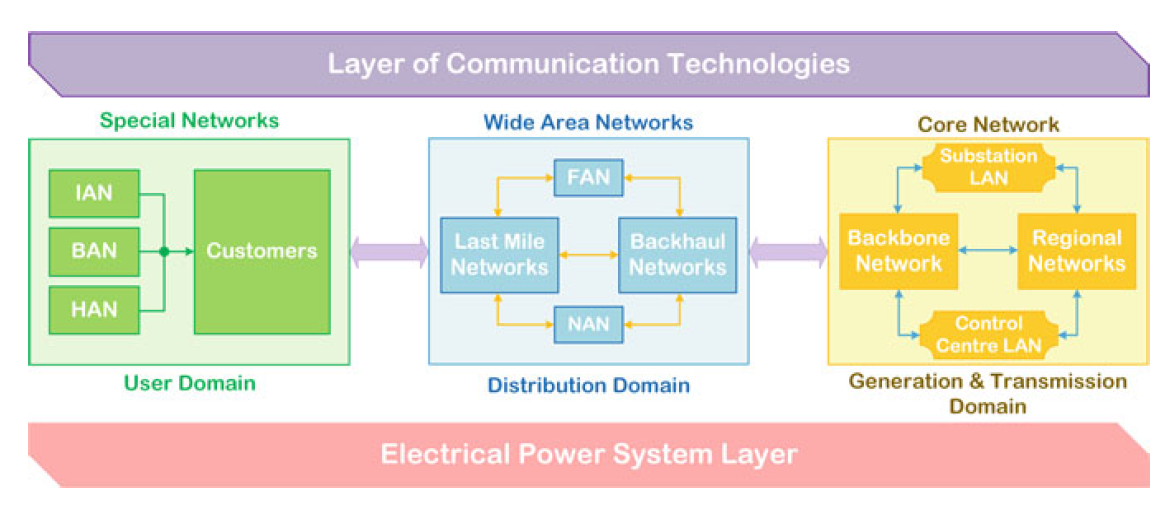
\includegraphics[width=\linewidth]{figures/IEEE2030-SG-CommunicationArchitecture.png}
\caption{The IEEE 2030 \acrlong{sg} Communication Architecture, as presented in \cite{Kabalci2019}}
\label{fig:IEEE2030-SG-CommunicationArchitecture}
\end{figure}


Figure \ref{fig:IEEE2030-SG-CommunicationArchitecture} shows the IEEE 2030 \acrlong{sg} Communication Architecture, as presented in \cite{Kabalci2019}.

As visualised by figure \ref{fig:IEEE2030-SG-CommunicationArchitecture} a number of area networks exists.

In the User Domain, the local network of customers, are interfacing with the following area networks: 
\begin{itemize}
\item \acrfull{han} for Private customers %Home area network (HAN)
\item \acrfull{ban} for Commercial customers %Building area network (BAN) 
\item \acrfull{ian} for Industrial customers %Industrial area network (IAN)
\end{itemize}

In the Distribution Domain, a \acrfull{wan} may contain both \acrfull{nan} and \acrfull{fan}. 
\begin{itemize}

\item \acrfull{nan} %neighborhood area network (NAN),
\item \acrfull{fan} %field area network (FAN)
\item \acrfull{wan}  %wide-area network (WAN)
\end{itemize}









Access to electrical power is regarded as part of the critical infrastructure of any modern society. 

 For instance, the European Union, in \cite[p.  L 345/81]{eu2008council} adds \textit{"Infrastructures and facilities for generation and transmission of
electricity in respect of supply electricity"} to the list of sectors to be considered \acrfull{eci} sectors.







As an example, the process of transforming the closed \acrshort{pg} to a online, or internet-connected, \acrshort{sg}, makes the Energy sector more dependant on \acrshort{ict}/\acrshort{telco}
The online \acrshort{sg} may serve as an example of a Cyber-Physical system, introduced next. 






\section{The transition to the Smart Grid} 
The transition of the \acrlong{pg} to the \acrlong{sg} transforms the Legacy electrical power distribution system into a modern dynamic infrastructure, enabling automated monitoring and control, as well as storage of electricity for future use. 


Additionally, the ability of controlling when to consume power, by selecting low-cost time periods, optimises the consumption of energy. 

%[ \fullcite{Kabalci2019} ]\\ 






While the classic Power Grid utilises serial lines for one way communication in order to control the infrastructure, the \acrlong{sg} utilises IP-based networking for bi-directional communication between producers, distributors and consumers. The bi-directional connections between the consumers and the Power Grid introduces a route from publicly available networks which may be used by malicious actors to perform a Cyber attack with the possible intention of destabilising society by shutting down the supply of electric power.\\ 




\subsection{The Smart Grid as a Cyber Physical System}

The \acrlong{sg} may be described as a Cyber-Physical system, where a physical system providing electrical flows connects four of the seven domains of the \acrshort{sg} (Transmission, Generation, Distribution, and Customer Domains), while the remaining three domains (Markets, Operations, and Service Provider Domains) are unique to the Cyber system. The Cyber system interconnects each of the seven domains, forming two-way network connections as required, for the purpose of monitoring, control and management of the \acrshort{sg}. \\







Figure \ref{fig:NIST-SmartGRID-Detailed-ConceptualModel} shows a detailed conceptual model of the smart grid.

\begin{figure}[ht]
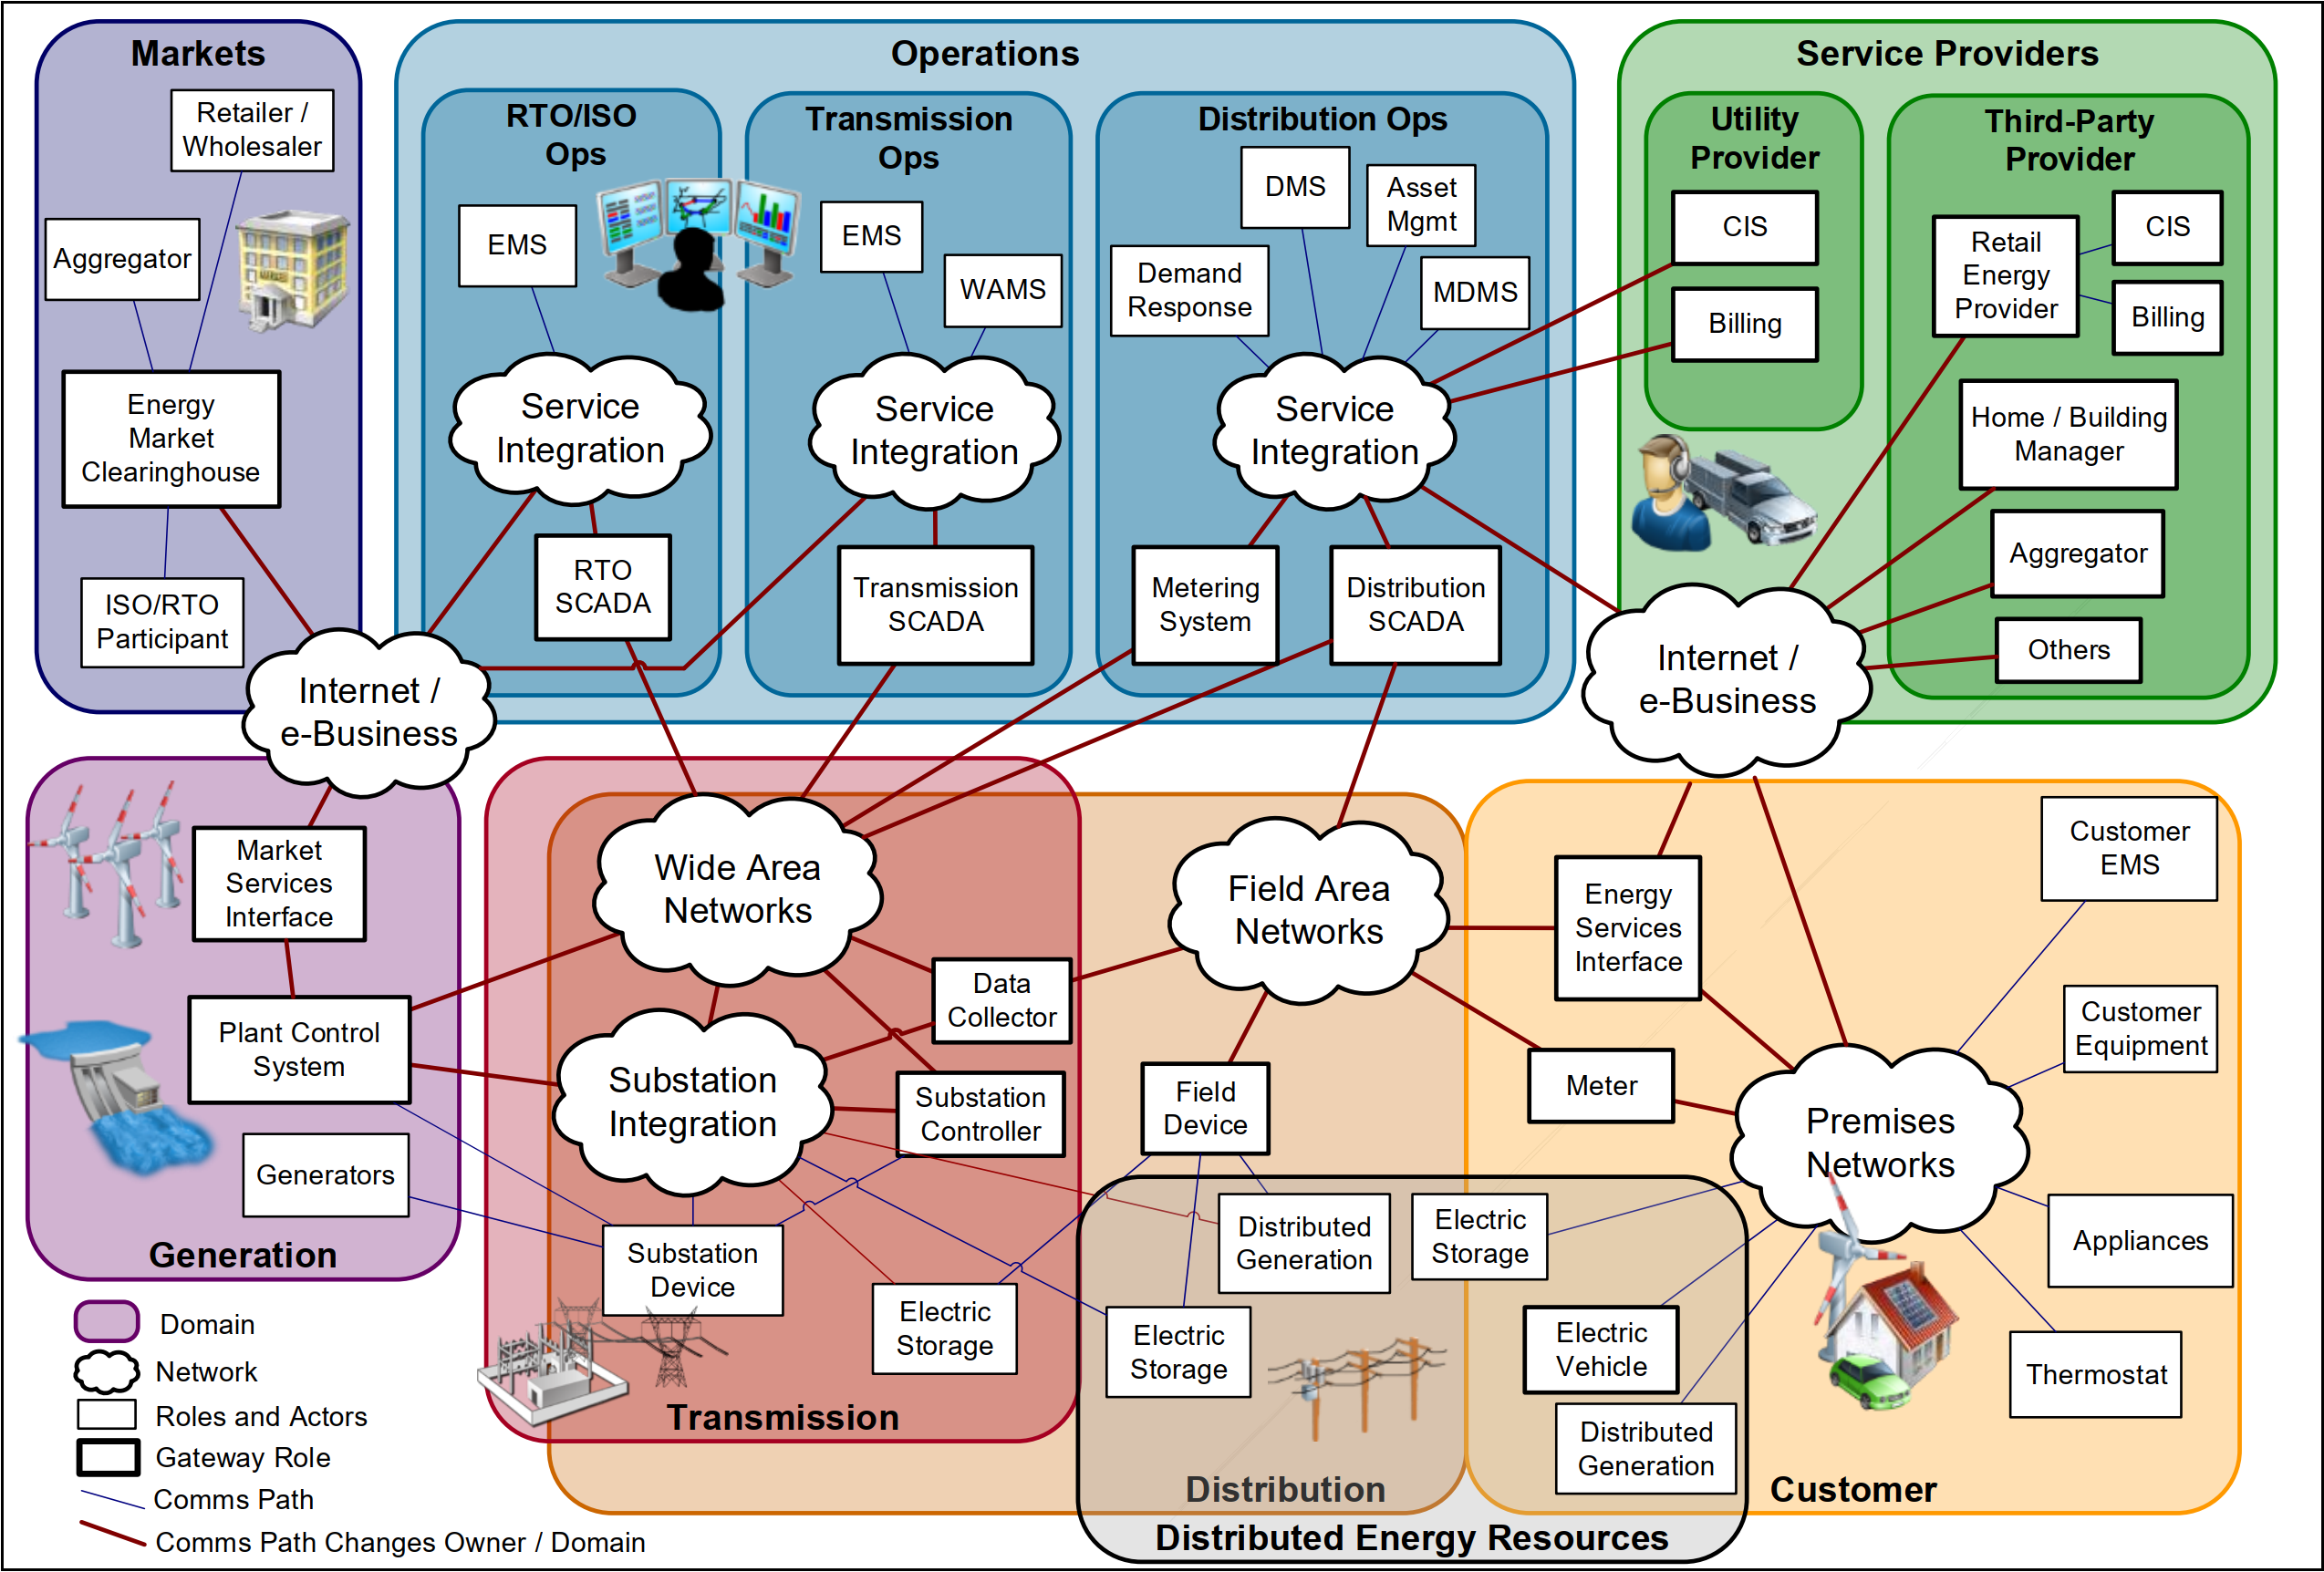
\includegraphics[width=\linewidth]{figures/NIST-SmartGRID-Detailed-ConceptualModel.png}
\caption{The detailed conceptual model of the smart grid, as presented in \cite{greer2014nist}}
\label{fig:NIST-SmartGRID-Detailed-ConceptualModel}
\end{figure}


%\ref{fig:NIST-SmartGRID-Detailed-ConceptualModel}





The conceptual model of the \acrshort{sg}, as shown in figure \ref{fig:NIST-SmartGRID-Detailed-ConceptualModel}, shows electrical flows and secure communication flows between the domains of the traditional power grid, as well as secure communication flows interconnecting the domains of the traditional power grid with the Markets, Operations, and Service Provider Domains, unique to the Smart Grid architecture.


Four of the Domains, the domains inherited from the classic \acrshort{pg}, are electrically connected, each of these four domains are electrically connected to at least two of the other electrically connected domains. The flow through the electrical connections, monitored and managed by secure communications channels, might be summarised as follows:

\begin{itemize}

\item The quality of the energy flow is Controlled by the Operations Domain, directly connected to every other domain by secure communication flows.  

\item The amount of energy generated is determined by demands controlled by the Markets domain.

\item Each of the electrically connected domains are electrically connected to every other electrically connected domains, apart from the Transmission Domain and Customer Domain, not being connected to each other by a direct electrical connection.

\item The Customer Domain consists of commercial and residential customers, electrically connected to the Distribution domain and Generation Domains. 

\item The \acrshort{pg} enables any Customer to include power producing facilities, like solar cells or wind turbines, to their local energy network, enabling a bi-directional energy flow, by consumers selling excessive energy to be distributed to other consumers, or storing the electricity for future used by charging electric vehicles.



\end{itemize}

In addition to the connections between the domains of the \acrshort{pg}, several secure communication flows ensures two-way communication flows, in order for the \acrshort{sg} to be monitored and controlled as required. 

\begin{itemize}
\item The \textbf{Operation} domain interconnects with every other domain, for \acrshort{sg} monitoring and management purposes.
\item The \textbf{Market} domain interconnects with every other domain, in order to obtain updated information regarding demand for and availability of power.
\item The \textbf{Service provider} domain interacts with every other domain, but the Distribution and Transmission domains. The transmission and distribution of electrical energy is monitored and serviced by the operations domain.
\end{itemize}

As described in \cite{wang2011survey}, each of the seven domain of the Smart Grid is connected to other domains as required in order to ensure a managed and monitored distribution of electrical energy in a reliable infrastructure. The connections between the domains may be categorised as electrical, for the purpose of energy distribution, or networked connections for communication purposes.




\section{Smart Grid Components}


%For monitoring and management purposes, a variety of bidirectional network connections interconnects the various domains, as described in \cite{wang2011survey}:

As described in \cite{Kabalci2019}, the \acrshort{sg} consists of a number of essential components:



\begin{enumerate}
    \item \textbf{Smart Sensors and Sensor Networks}
    \item \textbf{Phasor Measurement Units}
    \item \textbf{Smart Meters}
    \item \textbf{Wireless Sensor Networks}
    \end{enumerate}
\subsection{The Smart Grid Applications}
\begin{figure}[ht]
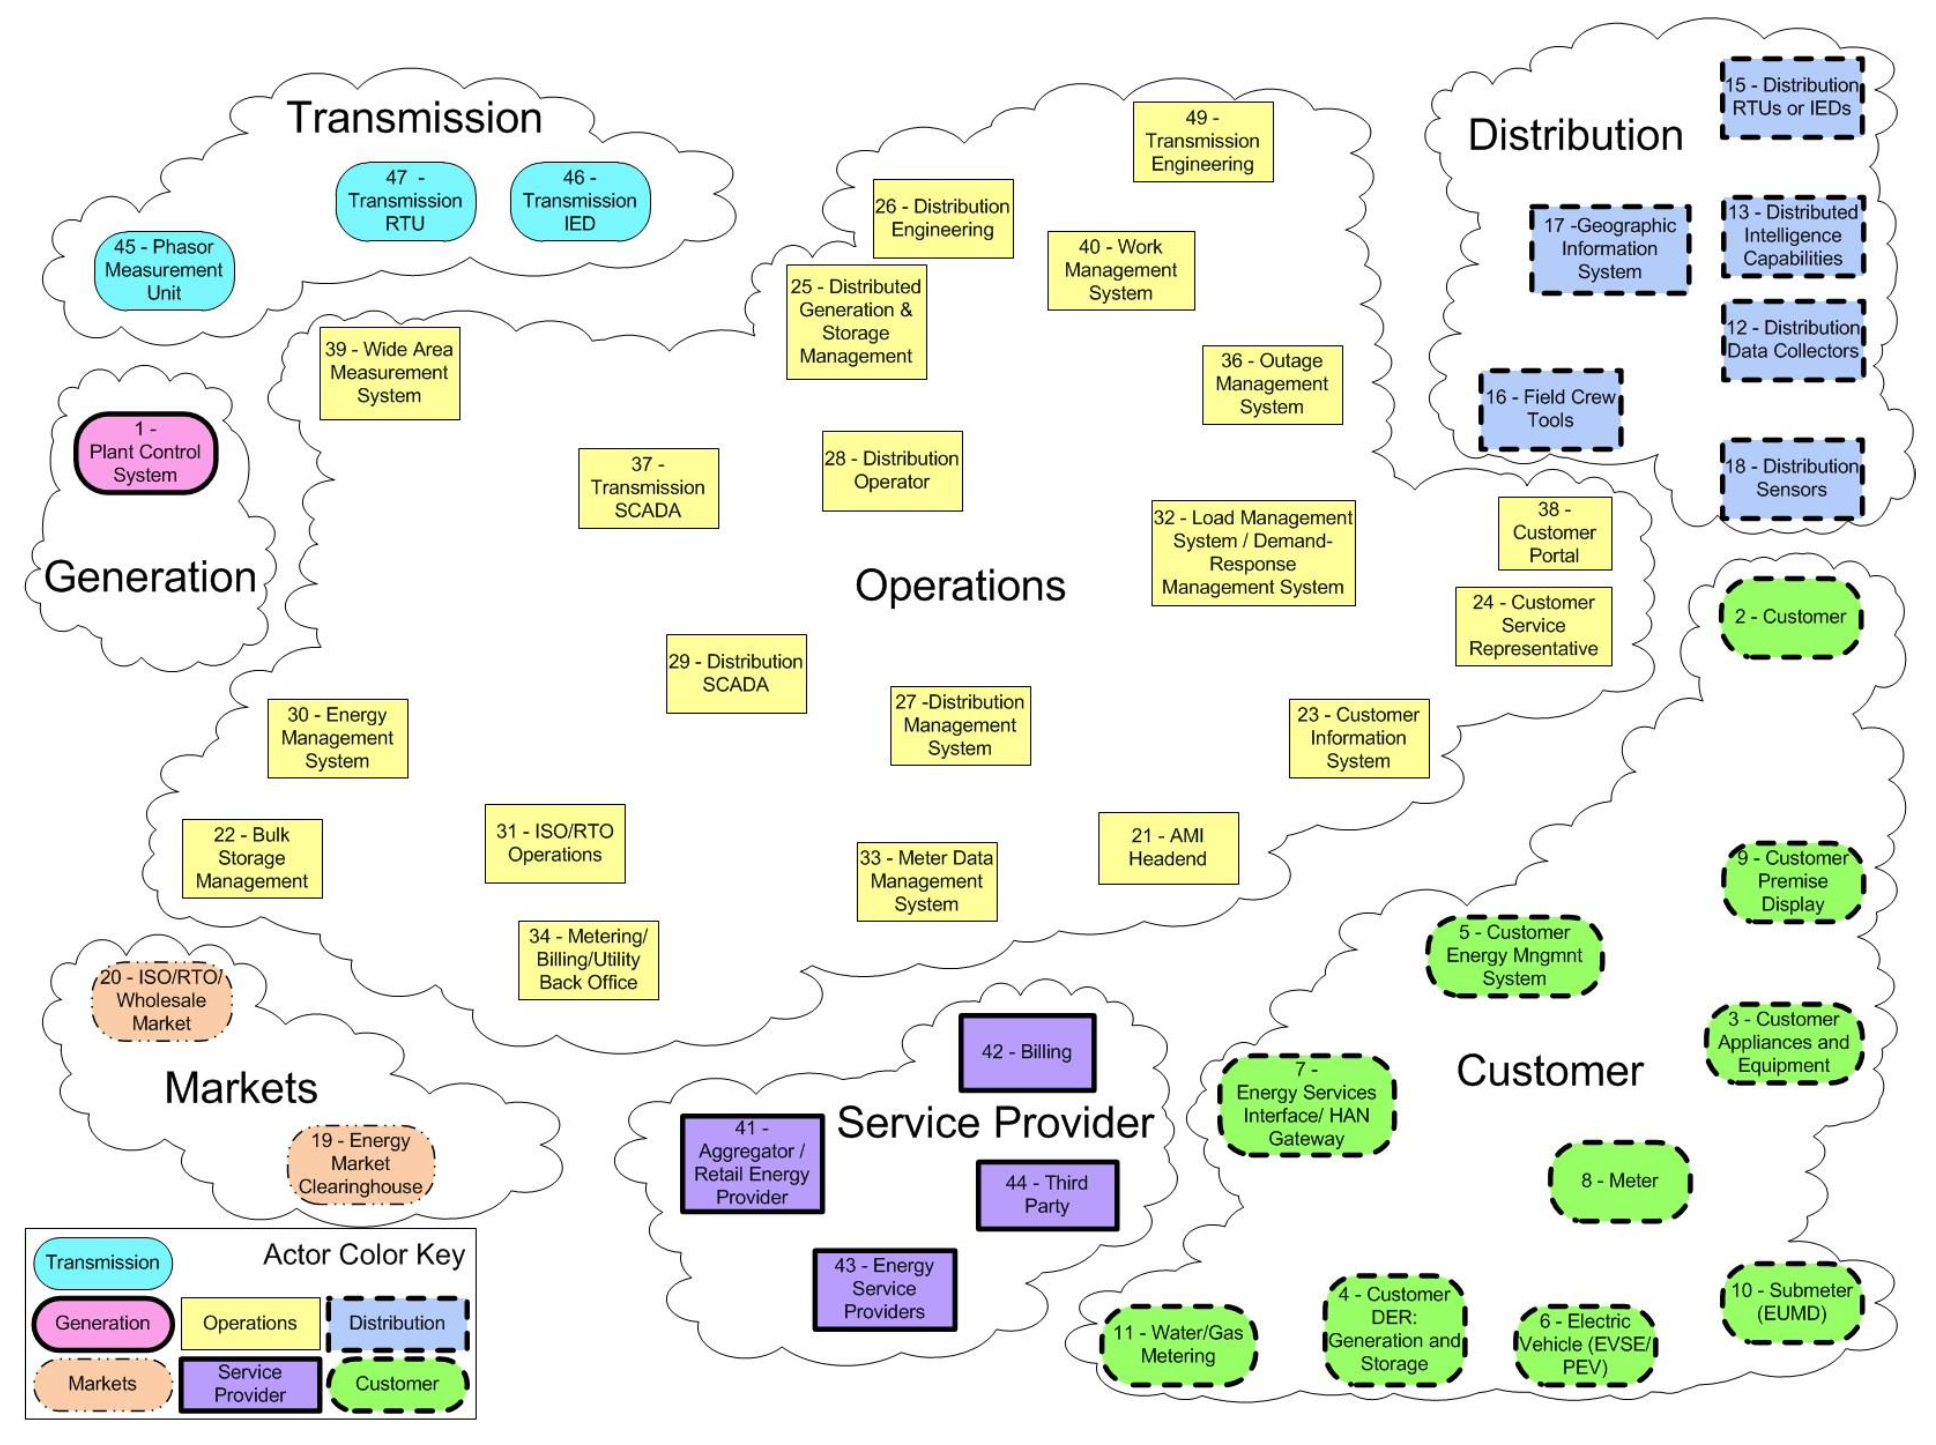
\includegraphics[width=\linewidth]{figures/NIST-Composite-High-level-View-of-the-Actors-within-Each-of-the-Smart-Grid-Domains.png}
\caption{The Composite High level View of the Actors within Each of the Smart Grid Domains, as presented by \cite{nist2010guidelines}} \label{fig:NIST-Composite-High-level-View-of-the-Actors-within-Each-of-the-Smart-Grid-Domains}
\end{figure}


\begin{enumerate}
    \item \textbf{Advanced Metering Infrastructures}
    \item \textbf{Demand Response}
    \item \textbf{Substation Automation Systems}
    \item \textbf{Demand-Side Management}

\end{enumerate}







A Control center component responsible for the monitoring of is the \acrfull{wams}.\\


Figure \ref{fig:Kumar-WAMS-architecture} shows the architecture of \acrshort{wams}, as presented by \cite{kumar2015monitoring}.

The \acrfull{wams} consists of a number of \acrfull{pdc} units, each getting samples from the locally connected \acrfull{pmu} units, costituting syncophasor data related to the status of power flow in the grid. The syncophasor data is associated with \acrfull{gps} time stamps, enabling the monitoring system to  relate data occuring in the same time slot to each other, enabling the system to display system-wide information related to \acrshort{sg} power flow status. 














\subsection{A comparison of the PG and SG characteristics}
A comparison of a selection of key characteristics of the power supply infrastructure, is listed in \cite{momoh2012smart}. For each characteristic selected, the  characteristics of the \acrlong{pg} is compared with  those of the \acrlong{sg}.





\begin{itemize}
    \item In order for the infrastructure to adhere to new requirements, \textbf{Active Consumer Participation} is vital in order adjust the amount of power required, in order to actual demand for power.

The \acrshort{pg} consumers are uninformed and do not participate in communication with the power supply provider\footnote{aside from the manual meter value reports periodically requested.}, while the \acrshort{sg} is classified by Informed, involved consumers demand response and distributed energy resources

\item \textbf{Accommodation of all generation and storage options}
The \acrshort{pg}  Dominated by central generation many obstacles exist for distributed energy resources interconnection , while the \acrshort{sg} Many distributed energy resources with plug-and-play convenience focus on renewables

\item \textbf{New products, services, and markets} 
The \acrshort{pg}  Limited, poorly integrated wholesale markets limited opportunities for consumers, while the \acrshort{sg} Mature, well-integrated wholesale markets growth of new electricity markets for consumers


\item \textbf{Provision of power quality for the digital economy} 
The \acrshort{pg} Focus on outages—slow response to power quality issues
, while the \acrshort{sg} Power quality a priority with a variety of quality/price options rapid resolution of issues 


\item \textbf{Optimization of assets and operates efficiently}
The \acrshort{pg} Little integration of operational data with asset management business process silos, while the \acrshort{sg} Greatly expanded data acquisition of grid parameters focus on prevention, minimizing impact to consumers 


\item \textbf{Anticipating responses to system disturbances (self-healing)}
The \acrshort{pg} Responds to prevent further damage focus on protecting assets following a fault, while the \acrshort{sg}

Automatically detects and responds to problems focus on prevention, minimizing impact to consumers 


\item \textbf{Resiliency against cyber attack and natural disasters} The \acrshort{pg}  Vulnerable to malicious acts of terror and natural disasters slow response, while the \acrshort{sg} Resilient to cyber attack and natural disasters rapid restoration capabilities 



\end{itemize}



%As described in \cite{rawat2015cyber}, these vulnerabilities vulnerabilities results in the following consequences:



%Electricity is produced in the Generation domain, by various means, like coal-based power plants, Nuclear power plants, or by reproducible sources like hydro-electric or wind energy power plants.




\subsection{Smart Grid Functional Requirements}


As presented by \cite{EnIndSecAct2007}, the \acrlong{sg} is characterised by the following demands for functionality:

\begin{enumerate}
\item Increased use of digital information and controls technology to improve reliability, security, and efficiency of the
electric grid.
\item Dynamic optimization of grid operations and resources,
with full cyber-security.
\item Deployment and integration of distributed resources
and generation, including renewable resources.
\item Development and incorporation of demand response,
demand-side resources, and energy-efficiency resources.
\item Deployment of ‘‘smart’’ technologies (real-time, automated, interactive technologies that optimize the physical operation of appliances and consumer devices) for metering, communications concerning grid operations and status, and distribution automation.
\item Integration of ‘‘smart’’ appliances and consumer devices.
\item Deployment and integration of advanced electricity storage and peak-shaving technologies, including plug-in electric
and hybrid electric vehicles, and thermal-storage air conditioning.
\item Provision to consumers of timely information and control
options.
\item Development of standards for communication and interoperability of appliances and equipment connected to the electric grid, including the infrastructure serving the grid.
\item Identification and lowering of unreasonable or unnecessary barriers to adoption of\acrlong{sg} technologies, practices,
and services. 

\end{enumerate}

In order to be able to adhere to demands like "demand response" and the "integration of ''smart'' appliances and consumer devices" the\acrlong{sg} requires connection to the Internet.\\









\subsection{The Smart Grid Control Center}
The \acrlong{sg} control center constitutes a distributed two-way monitoring, control and management infrastructure, communicating with various \acrlong{sg} subsystems, illustrated as the Operations subsystem of figure  \ref{fig:NIST-Composite-High-level-View-of-the-Actors-within-Each-of-the-Smart-Grid-Domains}



\cite{alcaraz2012security} describes the \acrlong{scada} system...















Figure \ref{fig:Blume-SCADA-system} shows the main components of the SCADA system.

\begin{figure}[ht]
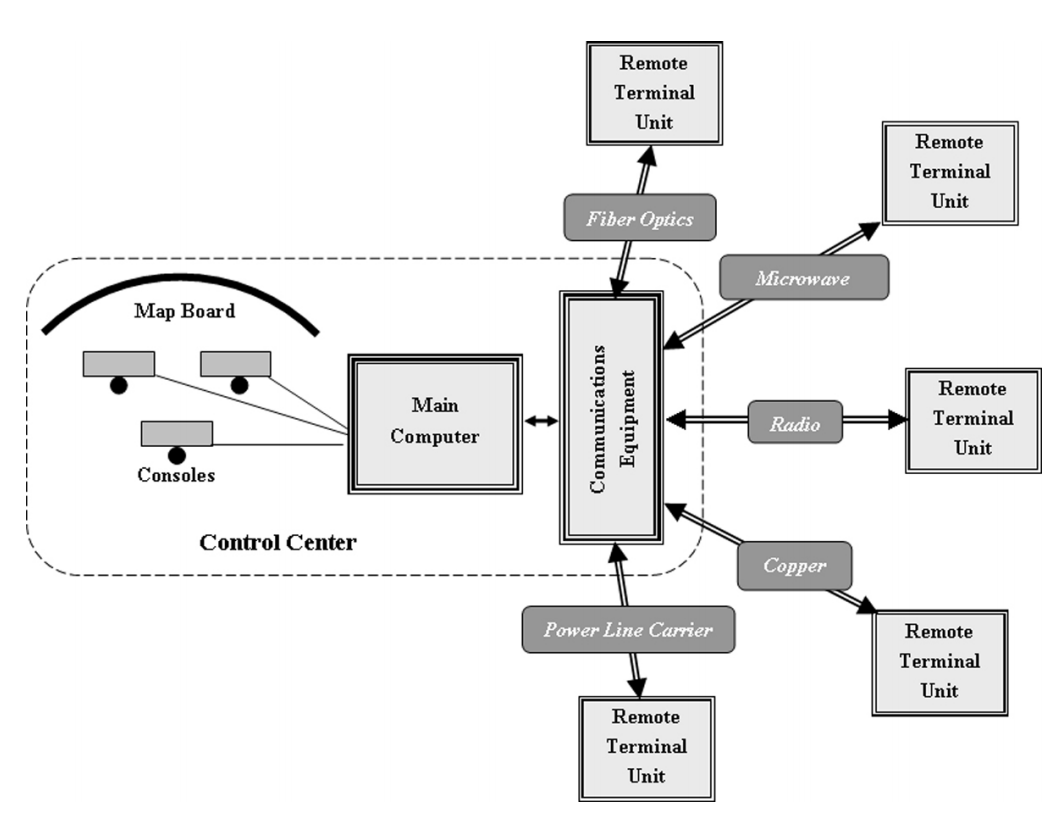
\includegraphics[width=\linewidth]{figures/Blume-SCADA-system.png}
\caption{SCADA system , as presented in \cite{BlumeStevenW2007Epsb}}
\label{fig:Blume-SCADA-system}
\end{figure}




In order to analyse previous attacks, as well as to avoid future attacks, models have been developed. 

\Cite{straub2020modeling}

%\subsubsection{The Diamond model}
 \subsubsection{MITRE ATT\&K framework}
 
 
 \Cite{strom2018mitre}
\subsubsection{STRIDE}

\cite{khan2017stride}
